\begin{tframe}{Duplicate Removal}

In the results of an image search engine there will be images that are \textbf{duplicates}, both because the returned links refer to the same location and because the same image is stored in two different locations. 

\vspace{0.1in}

In the created datasets there will be presents a certain number of duplicated images for each identity. 

\vspace{0.1in}

That is not desirable, since the dataset need to be used to train a \textbf{CNN}. A training phase need to generalized as much as possible the objects that is learning; a duplicated image does not add any useful information to this process.


\end{tframe}


\begin{tframe}{Duplicate Removal}

The images are represented as extended bounding boxes related to the detected faces, in order to consider not only the face but also the contest of the image.

\vspace{0.1in}

For each image, a \textbf{feature vector} is computed using the \textbf{Vector of Locally Aggregated Descriptor} (\textbf{VLAD}) encoding, using the implementation from the \textbf{VLFeat} library [5]. 

\vspace{0.1in}

The \textbf{VLAD} is a feature encoding and pooling method that encodes a set of local feature descriptors extracted from an image using a feature dictionary built using a clustering method. 

\vspace{0.1in}

These feature vectors are then \textbf{clustered} within the images for each identity; only a single element per cluster will be retained in order to removed the duplicated images.

\end{tframe}


\begin{tframe}{Duplicated Removal}

\begin{figure}[h]
\begin{center}
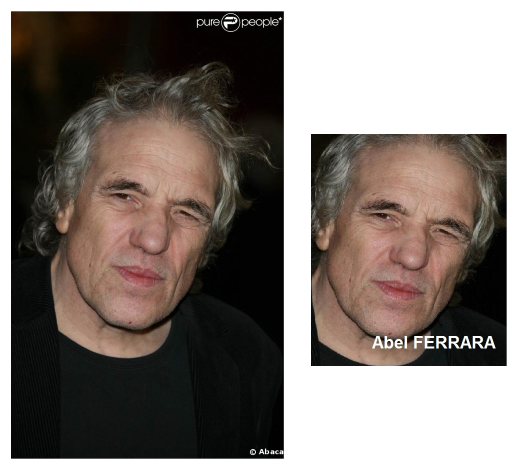
\includegraphics[width=0.55\textwidth]{images/image6.png}
\end{center}
  \caption{Example of two images, representing the same photo, but with different resolutions and scales so that the duplicate removal phase is not able see them as duplicates.}
\label{fig:validation}
\end{figure}

\end{tframe}